\documentclass[10pt,a4paper]{article}
\usepackage[utf8]{inputenc}
\usepackage[
    backend=biber,
    style=bwl-FU,
    url=false,
    doi=false,
    eprint=false]{biblatex}
\addbibresource{bibliography.bib}

%sections on new pages
\usepackage{titlesec}
\newcommand{\sectionbreak}{\clearpage}

\usepackage{amsmath}
\usepackage{amssymb}
\usepackage{graphicx}
\usepackage{threeparttable}
\usepackage{blindtext}
\usepackage{booktabs}
\usepackage{array}       
\usepackage{tabularx}
\usepackage{dcolumn} 
  \newcolumntype{d}[1]{D{.}{.}{#1}}    

\usepackage[table]{xcolor}
\usepackage{pgfplotstable}
\pgfplotsset{compat=1.17}
\pgfplotstableset{
    color cells/.style={
        col sep=comma,
        string type,
        postproc cell content/.code={%
                \pgfkeysalso{@cell content=\rule{0cm}{2.4ex}\cellcolor{red!##1}\pgfmathtruncatemacro\number{##1}\ifnum\number>50\color{white}\fi##1}%
                },
        columns/x/.style={
            column name={},
            postproc cell content/.code={}
        }
    }
}

\usepgfplotslibrary{colorbrewer}

\title{%
  Digital Tools for Finance \\
  \large What you should know!}
\author{Maximilian Weber\thanks{University of Zurich, Switzerland}\;\thanks{We are extremely grateful to Igor Pozdeev for his unwavering support and patient advice.} \\
\and David Jaggi\footnotemark[1]\;\footnotemark[2]}
\date{December 2021}

\begin{document}
\maketitle

\begin{abstract}
    \blindtext
\end{abstract}

\tableofcontents
\section{Introduction}
\blindtext[3]
\textcite{gormsenCoronavirusImpactStock2020}
\begin{figure}[h!]%
    \centering
    \includegraphics[width=6cm]{text/paper/github_logo.png}%
    \caption{GitHub Logo}%
    \footnotesize Numbers represent search interest relative to the highest point on the chart for the given region and time. A value of 100 is the peak popularity for the term. A value of 50 means that the term is half as popular. A score of 0 means there was not enough data for this term.
    \label{fig:github_logo}%
\end{figure}
\section{Methods}
\blindtext[3]
\textcite{kozlowskiTailThatWags2020}
\begin{table}
    \centering  
  \begin{threeparttable}
    \caption{Sample ANOVA table}
     \begin{tabular}{lllll}
        \toprule
        Stubhead & \( df \) & \( f \) & \( \eta \) & \( p \) \\
        \midrule
                 &     \multicolumn{4}{c}{Spanning text}     \\
        Row 1    & 1        & 0.67    & 0.55       & 0.41    \\
        Row 2    & 2        & 0.02    & 0.01       & 0.39    \\
        Row 3    & 3        & 0.15    & 0.33       & 0.34    \\
        Row 4    & 4        & 1.00    & 0.76       & 0.54    \\
        \bottomrule
     \end{tabular}
    \begin{tablenotes}
      \small
      \item Additional information on the data and methods used.
    \end{tablenotes}
  \end{threeparttable}
\end{table}
\section{Results}
\blindtext[1]
% table using D from dcolumn package
\begin{table}

  \centering
  \caption{Table with package dcolumn}
  \begin{tabularx}{\textwidth}{l*{3}{d{-2}}}
  \toprule
            &  \multicolumn{1}{X}{\centering col A} &
\multicolumn{1}{X}{\centering col B} &
\multicolumn{1}{X}{\centering col C} \\
\cmidrule(lr){2-2} \cmidrule(lr){3-3} \cmidrule(lr){4-4}
  \midrule  
       North &      2'228.0   &   0.3 &  10.6 \\    
       South &        689.2 &   0.8   &   2.6 \\
  \bottomrule

  \end{tabularx}     
\end{table}
\blindtext[1]
\begin{table}[ht]
    \caption{Table as a heatmap}
    \centering
    \pgfplotstabletypeset[color cells]{
    x,a,b,c,d
    a,90,10.5,0,0
    b,0,80,10,10
    c,0,0,95,5
    d,0,10,5,85
    }
\end{table}
\section{Discussion}
\blindtext[1]
\begin{figure}[ht]
    \caption{Line plot using colorbrewer}
    \centering
    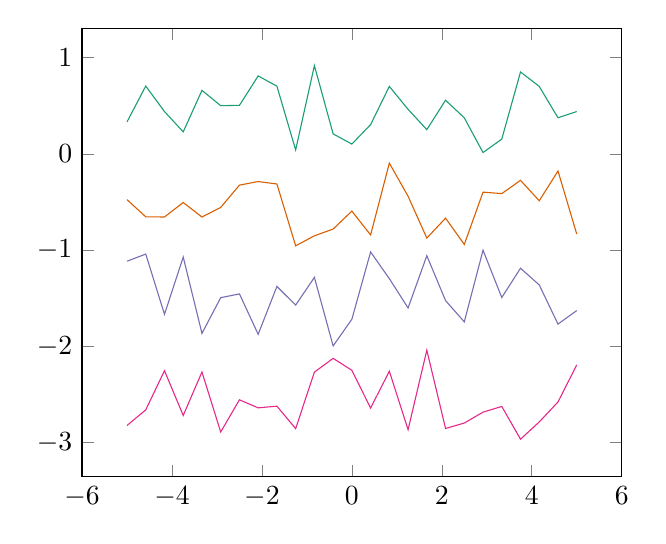
\begin{tikzpicture}
    \begin{axis}[
        cycle list/Dark2,
    ]
    \addplot {rnd};
    \addplot {rnd-1};
    \addplot {rnd-2};
    \addplot {rnd-3};
    
    \end{axis}
    \end{tikzpicture}
\end{figure}

\blindtext[1]

\printbibliography
\end{document}